\documentclass[14pt]{article}
\usepackage{url}
\usepackage{hyperref}
\usepackage{amsmath}
\usepackage{mathtools}
\usepackage{extsizes}
\usepackage{titling}
\usepackage{siunitx}
\usepackage{graphicx}
\usepackage[shortlabels]{enumitem}
\usepackage[margin=0.75in]{geometry}
\usepackage{indentfirst}
\usepackage{caption}

\newcommand{\bd}{\textbf}

\setlength{\droptitle}{-5em} 

\title{Written Homework 4}
\author{Mitchell Meier}
\date{\today}

\begin{document}

\maketitle

\begin{enumerate}

\item
\begin{enumerate}[(a)]
\item
\bd{Response Variable:} Battery Life, measured in hours

\item
\bd{Factor 1:} Material Type \\
\bd{Factor Levels:} Material 1, Material 2, Material 3 \\

\bd{Factor 2:} Temperature \\
\bd{Factor Levels:} 15$^{\circ}$F, 75$^{\circ}$F, 125$^{\circ}$F

\item
\bd{Number of Replications:} 4 replications per treatment combination, 36 replications total
\end{enumerate}
\vspace{2.5em}

\item
Check the assumption that population distributions are normal:
\begin{figure}[h]
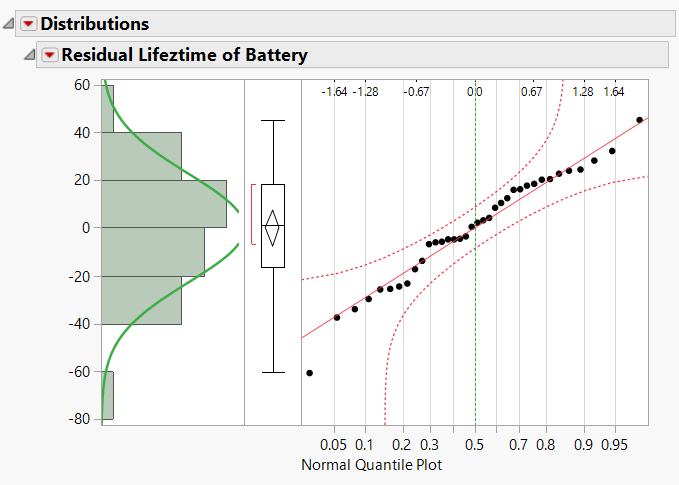
\includegraphics[scale=0.75]{hw4Pics/2-1.PNG}
\centering
\end{figure}

Shape of the distrubution resembles the shape of a normal distribution in the histogram, therefore making it safe to assume that the populations follow a normal distribution \\

Check the assumption that the population distributions have the same variance:
\begin{figure}[h]
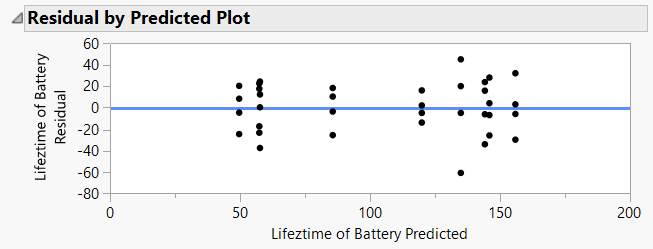
\includegraphics{hw4Pics/2-2.PNG}
\centering
\end{figure}
Residual plot values average out to around 0 and the residual plot shows no increasing or decreasing relations, therefore making it safe to assume that the populations have the same variance 
\vspace{1em}

\item
$H_0:$ Overall model is not significant \\
$H_1:$ Overall model is significant

\begin{figure}[h]
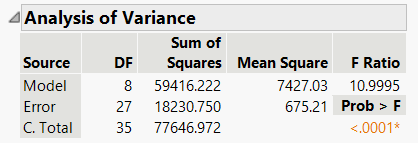
\includegraphics{hw4Pics/3-1.PNG}
\centering
\end{figure}

Our final p value for the model is evaluated at $< 0.0001$ \\
With our $\alpha$ value assumed to be 0.05, the p-value $< \alpha$, meaning we reject $H_0$ and can conclude our overall model is significant
\vspace{1em}

\item

As with our overall model, our p value for the interaction with tempature and material type is less than our significane level $\alpha$, meaning we can conclude that interaction is significant. Since an interaction with both of our main effects is significant, there is no reason to further test the main effects individually

\begin{figure}[h]
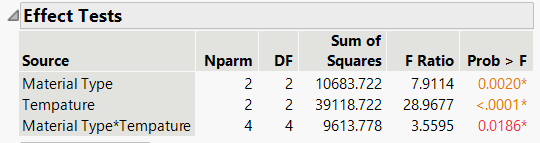
\includegraphics{hw4Pics/4-1.PNG}
\centering
\end{figure}




\end{enumerate}

\end{document}